% Options for packages loaded elsewhere
% Options for packages loaded elsewhere
\PassOptionsToPackage{unicode}{hyperref}
\PassOptionsToPackage{hyphens}{url}
%
\documentclass[
  ignorenonframetext,
  aspectratio=169,
]{beamer}
\newif\ifbibliography
\usepackage{pgfpages}
\setbeamertemplate{caption}[numbered]
\setbeamertemplate{caption label separator}{: }
\setbeamercolor{caption name}{fg=normal text.fg}
\beamertemplatenavigationsymbolsempty
% remove section numbering
\setbeamertemplate{part page}{
  \centering
  \begin{beamercolorbox}[sep=16pt,center]{part title}
    \usebeamerfont{part title}\insertpart\par
  \end{beamercolorbox}
}
\setbeamertemplate{section page}{
  \centering
  \begin{beamercolorbox}[sep=12pt,center]{section title}
    \usebeamerfont{section title}\insertsection\par
  \end{beamercolorbox}
}
\setbeamertemplate{subsection page}{
  \centering
  \begin{beamercolorbox}[sep=8pt,center]{subsection title}
    \usebeamerfont{subsection title}\insertsubsection\par
  \end{beamercolorbox}
}
% Prevent slide breaks in the middle of a paragraph
\widowpenalties 1 10000
\raggedbottom
\usepackage{iftex}
\ifPDFTeX
  \usepackage[T1]{fontenc}
  \usepackage[utf8]{inputenc}
  \usepackage{textcomp} % provide euro and other symbols
\else % if luatex or xetex
  \usepackage{unicode-math} % this also loads fontspec
  \defaultfontfeatures{Scale=MatchLowercase}
  \defaultfontfeatures[\rmfamily]{Ligatures=TeX,Scale=1}
\fi
\usepackage{lmodern}

\ifPDFTeX\else
  % xetex/luatex font selection
\fi
% Use upquote if available, for straight quotes in verbatim environments
\IfFileExists{upquote.sty}{\usepackage{upquote}}{}
\IfFileExists{microtype.sty}{% use microtype if available
  \usepackage[]{microtype}
  \UseMicrotypeSet[protrusion]{basicmath} % disable protrusion for tt fonts
}{}
\makeatletter
\@ifundefined{KOMAClassName}{% if non-KOMA class
  \IfFileExists{parskip.sty}{%
    \usepackage{parskip}
  }{% else
    \setlength{\parindent}{0pt}
    \setlength{\parskip}{6pt plus 2pt minus 1pt}}
}{% if KOMA class
  \KOMAoptions{parskip=half}}
\makeatother


\usepackage{longtable,booktabs,array}
\usepackage{calc} % for calculating minipage widths
\usepackage{caption}
% Make caption package work with longtable
\makeatletter
\def\fnum@table{\tablename~\thetable}
\makeatother
\usepackage{graphicx}
\makeatletter
\newsavebox\pandoc@box
\newcommand*\pandocbounded[1]{% scales image to fit in text height/width
  \sbox\pandoc@box{#1}%
  \Gscale@div\@tempa{\textheight}{\dimexpr\ht\pandoc@box+\dp\pandoc@box\relax}%
  \Gscale@div\@tempb{\linewidth}{\wd\pandoc@box}%
  \ifdim\@tempb\p@<\@tempa\p@\let\@tempa\@tempb\fi% select the smaller of both
  \ifdim\@tempa\p@<\p@\scalebox{\@tempa}{\usebox\pandoc@box}%
  \else\usebox{\pandoc@box}%
  \fi%
}
% Set default figure placement to htbp
\def\fps@figure{htbp}
\makeatother





\setlength{\emergencystretch}{3em} % prevent overfull lines

\providecommand{\tightlist}{%
  \setlength{\itemsep}{0pt}\setlength{\parskip}{0pt}}



 


% ============================================================
%  ECO 2203 — Beamer Metropolis Theme Preamble
%  Course: International Trade and Policy in Agriculture
%  Instructor: Nithin M, Department of Development Economics
% ============================================================

% MUST be first: load Metropolis theme before \metroset and colour overrides
\usetheme{metropolis}

% Only load packages not already provided by pandoc's beamer template
\usepackage{amsmath,amssymb}

% ---- Brand colours -----------------------------------------
\definecolor{brandblue}{HTML}{012169}
\definecolor{brandgold}{HTML}{B9975B}
\definecolor{lightblue}{HTML}{E8EDF5}

% ---- Metropolis colour overrides ---------------------------
% Main palette
\setbeamercolor{normal text}{fg=black,bg=white}
\setbeamercolor{alerted text}{fg=brandgold}
\setbeamercolor{example text}{fg=brandblue!70!black}

% Title slide
\setbeamercolor{title}{fg=white,bg=brandblue}
\setbeamercolor{subtitle}{fg=brandgold}
\setbeamercolor{author}{fg=white}
\setbeamercolor{institute}{fg=brandgold!80!white}
\setbeamercolor{date}{fg=white}
\setbeamercolor{title page header}{fg=white,bg=brandblue}

% Frametitle bar
\setbeamercolor{frametitle}{fg=white,bg=brandblue}

% Progress bar → gold
\setbeamercolor{progress bar}{fg=brandgold,bg=brandblue!30}
\setbeamercolor{title separator}{fg=brandgold}
\setbeamercolor{progress bar in head/foot}{fg=brandgold,bg=brandblue!20}
\setbeamercolor{progress bar in section page}{fg=brandgold,bg=brandblue!20}

% Blocks
\setbeamercolor{block title}{bg=brandblue,fg=white}
\setbeamercolor{block body}{bg=lightblue,fg=black}
\setbeamercolor{block title alerted}{bg=brandgold,fg=white}
\setbeamercolor{block body alerted}{bg=brandgold!12,fg=black}
\setbeamercolor{block title example}{bg=brandblue!70!black,fg=white}
\setbeamercolor{block body example}{bg=brandblue!8,fg=black}

% Structure / lists
\setbeamercolor{structure}{fg=brandblue}
\setbeamercolor{section in toc}{fg=brandblue}
\setbeamercolor{itemize item}{fg=brandblue}
\setbeamercolor{itemize subitem}{fg=brandgold}
\setbeamercolor{enumerate item}{fg=brandblue}
\setbeamercolor{description item}{fg=brandblue}

% ---- Metropolis options ------------------------------------
\metroset{
  progressbar    = frametitle,   % gold bar under frametitle
  sectionpage    = none,
  numbering      = fraction,
  block          = fill
}

% ---- Fonts (Metropolis uses Fira Sans; fallback gracefully) -
\setbeamerfont{title}{size=\Large,series=\bfseries}
\setbeamerfont{subtitle}{size=\normalsize,series=\mdseries}
\setbeamerfont{frametitle}{size=\large,series=\bfseries}
\setbeamerfont{block title}{size=\normalsize,series=\bfseries}
\setbeamerfont{caption}{size=\footnotesize}

% ---- Footer: course info + slide number --------------------
\setbeamertemplate{footline}{%
  \begin{beamercolorbox}[wd=\paperwidth,ht=2.0ex,dp=1ex]{footline}%
    \hspace{0.8em}%
    {\footnotesize\color{brandblue!60}%
      ECO 2203 \textbar{} International Trade and Policy in Agriculture
      \hfill Nithin M \hfill
      \insertframenumber{}/\inserttotalframenumber\hspace{0.8em}}%
  \end{beamercolorbox}%
}

% ---- Misc --------------------------------------------------
\setlength{\parskip}{0.25em}
\setbeamertemplate{navigation symbols}{}

% tighter column sep for side-by-side content
\setlength{\columnsep}{0.8em}

% Fix: make \label truly robust in moving arguments (Quarto generates
% \caption{\label{fig-xxx}...} which crashes Metropolis in batchmode).
% DeclareRobustCommand creates a self-protecting robust version.
\makeatletter
\let\quarto@originallabel\label
\DeclareRobustCommand*{\label}[1]{\quarto@originallabel{#1}}
\makeatother

% Prevent figures from overflowing Beamer frames.
% width=\linewidth: scale to text width (already Quarto default);
% height=0.6\textheight: cap height so figures never push past the frame bottom.
% keepaspectratio: never distort — whichever constraint binds first wins.
\setkeys{Gin}{width=\linewidth,height=0.6\textheight,keepaspectratio}
\makeatletter
\@ifpackageloaded{caption}{}{\usepackage{caption}}
\AtBeginDocument{%
\ifdefined\contentsname
  \renewcommand*\contentsname{Table of contents}
\else
  \newcommand\contentsname{Table of contents}
\fi
\ifdefined\listfigurename
  \renewcommand*\listfigurename{List of Figures}
\else
  \newcommand\listfigurename{List of Figures}
\fi
\ifdefined\listtablename
  \renewcommand*\listtablename{List of Tables}
\else
  \newcommand\listtablename{List of Tables}
\fi
\ifdefined\figurename
  \renewcommand*\figurename{Figure}
\else
  \newcommand\figurename{Figure}
\fi
\ifdefined\tablename
  \renewcommand*\tablename{Table}
\else
  \newcommand\tablename{Table}
\fi
}
\@ifpackageloaded{float}{}{\usepackage{float}}
\floatstyle{ruled}
\@ifundefined{c@chapter}{\newfloat{codelisting}{h}{lop}}{\newfloat{codelisting}{h}{lop}[chapter]}
\floatname{codelisting}{Listing}
\newcommand*\listoflistings{\listof{codelisting}{List of Listings}}
\makeatother
\makeatletter
\makeatother
\makeatletter
\@ifpackageloaded{caption}{}{\usepackage{caption}}
\@ifpackageloaded{subcaption}{}{\usepackage{subcaption}}
\makeatother

\usepackage{bookmark}
\IfFileExists{xurl.sty}{\usepackage{xurl}}{} % add URL line breaks if available
\urlstyle{same}
\hypersetup{
  pdftitle={Theories of International Trade I},
  pdfauthor={Nithin M},
  hidelinks,
  pdfcreator={LaTeX via pandoc}}


\title{Theories of International Trade I}
\subtitle{ECO 2203 \textbar{} International Trade and Policy in
Agriculture}
\author{Nithin M}
\date{2026-05-09}
\institute{Department of Development Economics}

\begin{document}
\frame{\titlepage}


\section{Part I: The Central
Question}\label{part-i-the-central-question}

\begin{frame}{The Central Question}
\phantomsection\label{the-central-question}
\begin{columns}[T]
\begin{column}{0.6\linewidth}
\textbf{Why do countries trade?}

This question has occupied economists for over 500 years. Three broad
answers have emerged:

\begin{enumerate}
\tightlist
\item
  \textbf{Mercantilism (1500--1750):} Trade is a zero-sum competition
  for power; exports = good, imports = bad; accumulate gold
\end{enumerate}

\begin{enumerate}
\setcounter{enumi}{1}
\tightlist
\item
  \textbf{Absolute Advantage --- Adam Smith (1776):} Trade is win-win;
  each country specialises in what it produces \emph{most efficiently}
\end{enumerate}

\begin{enumerate}
\setcounter{enumi}{2}
\tightlist
\item
  \textbf{Comparative Advantage --- David Ricardo (1817):} Even if one
  country is better at \emph{everything}, both countries gain from trade
  based on \emph{relative} costs
\end{enumerate}
\end{column}

\begin{column}{0.4\linewidth}
\textbf{Why theory matters for policy}

India bans rice exports → mercantilist instinct (protect domestic
supply, accumulate foreign exchange from \emph{other} goods)

India signs FTAs → comparative advantage logic (specialise and exchange)

These theories are not just history --- they are the intellectual
foundation of every trade policy debate happening right now.
\end{column}
\end{columns}
\end{frame}

\begin{frame}{Overview of Trade Theories: A Timeline}
\phantomsection\label{overview-of-trade-theories-a-timeline}
\begin{longtable}[]{@{}
  >{\raggedright\arraybackslash}p{(\linewidth - 6\tabcolsep) * \real{0.1860}}
  >{\raggedright\arraybackslash}p{(\linewidth - 6\tabcolsep) * \real{0.2093}}
  >{\raggedright\arraybackslash}p{(\linewidth - 6\tabcolsep) * \real{0.2326}}
  >{\raggedright\arraybackslash}p{(\linewidth - 6\tabcolsep) * \real{0.3721}}@{}}
\toprule\noalign{}
\begin{minipage}[b]{\linewidth}\raggedright
Period
\end{minipage} & \begin{minipage}[b]{\linewidth}\raggedright
Theory
\end{minipage} & \begin{minipage}[b]{\linewidth}\raggedright
Key Idea
\end{minipage} & \begin{minipage}[b]{\linewidth}\raggedright
Main Proponent
\end{minipage} \\
\midrule\noalign{}
\endhead
1500--1750 & \textbf{Mercantilism} & Wealth = gold; maximise trade
surplus & Colbert, Mun \\
1776 & \textbf{Absolute Advantage} & Specialise where you are
\emph{most} productive & Adam Smith \\
1817 & \textbf{Comparative Advantage} & Specialise where you have
\emph{lowest opportunity cost} & David Ricardo \\
1933 & \textbf{Factor Endowments (H-O)} & Trade reflects relative factor
abundance & Heckscher, Ohlin \\
1953 & \textbf{Leontief Paradox} & Empirical challenge to H-O &
Leontief \\
1970s--80s & \textbf{New Trade Theory} & Economies of scale + imperfect
competition & Krugman \\
1990s & \textbf{Porter's Diamond} & Competitive advantage of nations &
Porter \\
2000s & \textbf{New New Trade Theory} & Firm-level heterogeneity in
trade & Melitz \\
\bottomrule\noalign{}
\end{longtable}

Each theory addresses a limitation of the previous one. By Lecture 6, we
will have covered the full arc. Today: mercantilism and Smith.
\end{frame}

\section{Part II: Mercantilism}\label{part-ii-mercantilism}

\begin{frame}{What is Mercantilism?}
\phantomsection\label{what-is-mercantilism}
\begin{columns}[T]
\begin{column}{0.55\linewidth}
\textbf{Historical context}

\begin{itemize}
\tightlist
\item
  Dominant European trade doctrine: approximately 1500--1750 CE
\item
  Era of nation-state formation, colonial expansion, and bullion-based
  monetary systems
\item
  Gold and silver = the only ``real'' wealth; paper money not yet
  trusted
\end{itemize}

\textbf{Core beliefs of mercantilism}

\begin{itemize}
\tightlist
\item
  \textbf{Wealth of a nation = stock of gold and silver} it accumulates
\item
  To accumulate gold → \textbf{export more than you import} → trade
  surplus → gold flows in
\item
  Trade is \textbf{zero-sum:} one country's gain is another's loss
\item
  \textbf{State's role:} Actively promote exports, restrict imports,
  grant monopolies to favoured companies
\end{itemize}
\end{column}

\begin{column}{0.45\linewidth}
\textbf{Key mercantilist idea:}

\emph{``A nation is rich when it has more gold than other nations.''}

This view seems obvious to policymakers even today --- which is why
understanding and \emph{refuting} it is so important.

\textbf{Modern echo:} When Indian politicians say ``we must increase our
trade surplus,'' they are (often unknowingly) invoking mercantilist
logic.
\end{column}
\end{columns}
\end{frame}

\begin{frame}{Mercantilist Policies in Practice}
\phantomsection\label{mercantilist-policies-in-practice}
\begin{columns}[T]
\begin{column}{0.5\linewidth}
\textbf{Export promotion}

\begin{itemize}
\tightlist
\item
  \textbf{Export subsidies} --- government pays domestic producers to
  lower their export price
\item
  \textbf{State-supported trading companies} --- British East India
  Company (1600), Dutch VOC (1602): chartered monopolies given exclusive
  rights to trade with Asia
\item
  \textbf{Navigation Acts (England, 1651):} Required all trade to be
  carried in English ships → protect English shipping industry and
  exclude Dutch competition
\end{itemize}

\textbf{Import restriction}

\begin{itemize}
\tightlist
\item
  \textbf{High import tariffs} --- make foreign goods expensive
\item
  \textbf{Import bans/prohibitions} --- on manufactured goods that
  competed with domestic industries
\item
  \textbf{Colonialism} --- acquire raw material sources and captive
  markets for manufactured goods
\end{itemize}
\end{column}

\begin{column}{0.5\linewidth}
\textbf{Evaluation of mercantilist instruments}

\begin{longtable}[]{@{}
  >{\raggedright\arraybackslash}p{(\linewidth - 4\tabcolsep) * \real{0.1633}}
  >{\raggedright\arraybackslash}p{(\linewidth - 4\tabcolsep) * \real{0.4490}}
  >{\raggedright\arraybackslash}p{(\linewidth - 4\tabcolsep) * \real{0.3878}}@{}}
\toprule\noalign{}
\begin{minipage}[b]{\linewidth}\raggedright
Policy
\end{minipage} & \begin{minipage}[b]{\linewidth}\raggedright
Mercantilist rationale
\end{minipage} & \begin{minipage}[b]{\linewidth}\raggedright
Modern equivalent
\end{minipage} \\
\midrule\noalign{}
\endhead
Export subsidies & Increase gold inflow & India's RoDTEP, MEIS \\
Import duties & Keep gold in country & India's import tariff schedule \\
State monopolies & Control strategic trade & MMTC, STC trading houses \\
Colonial extraction & Secure raw materials & Resource-seeking FDI \\
Currency undervaluation & Make exports cheap & China 2000s, ``currency
manipulation'' debate \\
\bottomrule\noalign{}
\end{longtable}

Mercantilism was not entirely irrational --- for a small open economy
trying to industrialise, some ``mercantilist'' policies (infant industry
protection, export subsidies) may be justified. The \emph{error} is the
zero-sum worldview.
\end{column}
\end{columns}
\end{frame}

\begin{frame}{Colonial Trade: The Institutional Structure}
\phantomsection\label{colonial-trade-the-institutional-structure}
\begin{columns}[T]
\begin{column}{0.55\linewidth}
\textbf{British mercantilism in India}

\begin{itemize}
\tightlist
\item
  India was Britain's most valuable colonial possession --- primary
  purpose: source raw materials, provide captive market for British
  manufactures
\item
  \textbf{Raw material extraction:} Raw cotton from India → Manchester
  mills → cotton textiles back to India
\item
  \textbf{De-industrialisation:} India's famous cotton textile industry
  (Dhaka muslin, Surat cotton) was systematically destroyed through:

  \begin{itemize}
  \tightlist
  \item
    Zero/low import duties on British textiles entering India
  \item
    High export duties on Indian textiles entering Britain
  \item
    Physical destruction of Indian weavers' looms (disputed but
    documented in some accounts)
  \end{itemize}
\end{itemize}
\end{column}

\begin{column}{0.45\linewidth}
\textbf{The numbers (Utsa Patnaik, 2018 estimate)}

India transferred \textbf{\$45 trillion} to Britain between 1765 and
1938 (present-value estimate --- debated but widely cited).

Even conservative estimates show that India's per capita income
\emph{fell} under British rule --- from \textasciitilde comparable with
Britain in 1700 to less than 20\% of British levels by 1947.

\textbf{Agricultural dimension:} India was forced to grow indigo, opium,
and jute for British export markets rather than food crops → contributed
to famines (Bengal 1943: 2--3 million deaths)
\end{column}
\end{columns}
\end{frame}

\begin{frame}{The Drain of Wealth: Naoroji's Evidence}
\phantomsection\label{the-drain-of-wealth-naorojis-evidence}
\begin{columns}[T]
\begin{column}{0.55\linewidth}
\textbf{Dadabhai Naoroji's Drain Theory}

\begin{itemize}
\tightlist
\item
  Naoroji (1901): \emph{Poverty and Un-British Rule in India}
\item
  Calculated that Britain extracted \textbf{£200--300 million per year}
  from India as ``drain''
\item
  Home charges: India paid for British administration costs, interest on
  British-held debt, railway profits
\item
  The mechanism: India exported goods but received paper IOUs rather
  than gold --- a systematic wealth transfer disguised as trade
\item
  Silver drained from India → monetary contraction → deflation →
  economic stagnation
\end{itemize}
\end{column}

\begin{column}{0.45\linewidth}
``England has impoverished India by her own prosperity.'' --- Dadabhai
Naoroji, 1901

\textbf{Modern reassessment:} Economists Utsa Patnaik (2018) and Sashi
Tharoor (\emph{Inglorious Empire}, 2017) updated Naoroji's estimates.
The drain theory remains contested on methodology but its directional
conclusion --- that colonial trade systematically transferred wealth
from India to Britain --- is broadly accepted.
\end{column}
\end{columns}
\end{frame}

\begin{frame}{Critique of Mercantilism}
\phantomsection\label{critique-of-mercantilism}
\begin{columns}[T]
\begin{column}{0.55\linewidth}
\textbf{David Hume's price-specie-flow mechanism (1752)}

Mercantilism has a self-defeating logic:

\begin{enumerate}
\tightlist
\item
  Country A runs a trade surplus → gold flows in → money supply rises
\item
  More money → prices rise (quantity theory of money: MV = PQ)
\item
  Higher prices → Country A's exports become more expensive
\item
  Exports fall, imports rise → trade surplus disappears automatically
\item
  Gold flows back out
\end{enumerate}

\textbf{Conclusion:} A trade surplus is \emph{self-correcting};
mercantilist attempts to maintain it permanently are futile and cause
inflation.

\textbf{Adam Smith's critique (1776)}

\begin{itemize}
\tightlist
\item
  ``Wealth of a nation is not measured by the gold in its vaults but by
  the goods and services it can produce and consume''
\item
  Trade is \textbf{not zero-sum} --- both countries gain from
  specialisation
\item
  Import restrictions reduce the nation's consumption possibilities
\end{itemize}
\end{column}

\begin{column}{0.45\linewidth}
\textbf{The fundamental error of mercantilism}

Mercantilists confused the \textbf{means} (gold) with the \textbf{end}
(well-being of citizens).

A country with more gold but fewer goods and services is \emph{poorer},
not richer.

Smith's insight: A nation is wealthy when it has a \emph{high standard
of living} --- access to abundant, diverse, and cheap goods and
services. This requires \emph{imports}, not just exports.

\textbf{Modern parallel:} Japan in the 1980s ran huge trade surpluses
with the USA. Was Japan richer for it? Its citizens had high savings but
\emph{lower consumption} than Americans with similar incomes --- a
classic mercantilist outcome.
\end{column}
\end{columns}
\end{frame}

\begin{frame}{Mercantilist Arithmetic: Why the Logic Fails}
\phantomsection\label{mercantilist-arithmetic-why-the-logic-fails}
\textbf{The mercantilist objective function}

A nation seeks to accumulate gold \(G\) by maximising its trade surplus:

\[\text{Objective: } \max\; G = X - M\]

\[\Rightarrow \text{policy prescriptions: } X \uparrow \text{ (export subsidies)}, \quad M \downarrow \text{ (tariffs, prohibitions, bans)}\]

\begin{columns}[T]
\begin{column}{0.5\linewidth}
\textbf{The zero-sum fallacy}

If \emph{all} \(N\) nations simultaneously pursue a surplus:

\[\sum_{i=1}^{N}(X_i - M_i) = 0 \quad \forall \text{ nations simultaneously}\]

Every export is someone else's import --- the global sum of trade
balances is always exactly zero. Mercantilist policies merely
\emph{redistribute} gold among nations; they cannot increase the world's
total gold stock.
\end{column}

\begin{column}{0.5\linewidth}
\textbf{Hume's price-specie-flow refutation (1752)}

Even a single nation's surplus is self-correcting:

\[\text{Gold inflow} \;\Rightarrow\; M_s \uparrow \;\Rightarrow\; P \uparrow \;\Rightarrow\; X \downarrow,\; M \uparrow \;\Rightarrow\; \text{surplus eliminated}\]

Via the quantity theory of money (\(MV = PQ\), with \(V, Q\) fixed in
the short run):

\[\Delta G > 0 \;\Rightarrow\; \Delta M_s > 0 \;\Rightarrow\; P \uparrow \;\Rightarrow\; \text{exports become uncompetitive}\]

A mercantilist surplus is self-defeating: the very gold inflow it
generates raises domestic prices, eroding the export competitiveness
that created the surplus.
\end{column}
\end{columns}
\end{frame}

\begin{frame}{Smith's Critique: Real Wealth vs Gold}
\phantomsection\label{smiths-critique-real-wealth-vs-gold}
\textbf{Smith's fundamental restatement}

Mercantilists measured national wealth by the gold stock. Smith showed
the correct measure is real consumption:

\[W_{\text{real}} = \frac{\text{goods and services consumed}}{P} \;\neq\; \text{gold stock}\]

\begin{columns}[T]
\begin{column}{0.55\linewidth}
\textbf{The trade restriction paradox --- applied to India}

If India bans rice exports to keep supply at home:

\[W_{\text{domestic,rice}} \uparrow \quad \text{(rice cheaper domestically)}\]
\[W_{\text{global}} = 0 \quad \text{(no new rice created — redistributed, not added)}\]

If instead India exports rice and specialises:

\[W_{\text{global}} \uparrow \quad \text{(specialisation gains; world output expands)}\]
\[W_{\text{India}} \uparrow \quad \text{(farmers earn more; import cheaper goods)}\]

\textbf{The mercantilist error:} treating the \emph{means} (gold,
foreign exchange) as the \emph{end} (citizen well-being). A nation with
a large foreign exchange reserve but poor citizens has confused
instrument with objective.
\end{column}

\begin{column}{0.45\linewidth}
\textbf{Smith on imports}

\begin{quote}
\emph{``It is the maxim of every prudent master of a family, never to
attempt to make at home what it will cost him more to make than to
buy.''} --- Wealth of Nations, Book IV, Ch. 2
\end{quote}

Import restrictions are equivalent to a household refusing to buy
\emph{anything} from neighbours --- the household makes everything
itself, poorly and expensively, in the name of ``self-sufficiency.''

National self-sufficiency achieved through restriction destroys, not
creates, real wealth.
\end{column}
\end{columns}
\end{frame}

\begin{frame}{Mercantilism vs Smith: Policy Implications}
\phantomsection\label{mercantilism-vs-smith-policy-implications}
\begin{longtable}[]{@{}
  >{\raggedright\arraybackslash}p{(\linewidth - 4\tabcolsep) * \real{0.3333}}
  >{\raggedright\arraybackslash}p{(\linewidth - 4\tabcolsep) * \real{0.3333}}
  >{\raggedright\arraybackslash}p{(\linewidth - 4\tabcolsep) * \real{0.3333}}@{}}
\toprule\noalign{}
\begin{minipage}[b]{\linewidth}\raggedright
Dimension
\end{minipage} & \begin{minipage}[b]{\linewidth}\raggedright
Mercantilism
\end{minipage} & \begin{minipage}[b]{\linewidth}\raggedright
Adam Smith
\end{minipage} \\
\midrule\noalign{}
\endhead
\textbf{Goal} & National power / gold accumulation & National prosperity
/ consumption \\
\textbf{View of trade} & Zero-sum: one nation's gain = another's loss &
Positive-sum: specialisation grows world output \\
\textbf{Role of imports} & Evil --- gold drains out & Beneficial ---
access to cheaper goods \\
\textbf{Role of exports} & Good --- gold flows in & A means to pay for
imports \\
\textbf{State role} & Regulate all trade; grant monopolies &
Laissez-faire; let markets direct resources \\
\textbf{India example (2023)} & Rice/wheat export ban --- hoard grain,
protect prices & RCEP/FTA participation --- specialise, exchange \\
\bottomrule\noalign{}
\end{longtable}

\textbf{The modern policy echo:} Every time an Indian policymaker
imposes an export ban to protect domestic consumers, they invoke
mercantilist logic. Every time an economist argues for free trade to
raise farmer incomes, they invoke Smith. Both impulses co-exist in
India's agricultural trade policy --- understanding the theory clarifies
which logic applies when.
\end{frame}

\begin{frame}{Neo-Mercantilism: Export-Led Development Strategies}
\phantomsection\label{neo-mercantilism-export-led-development-strategies}
\begin{columns}[T]
\begin{column}{0.55\linewidth}
\textbf{Modern mercantilist practices}

\begin{itemize}
\tightlist
\item
  \textbf{Export-led growth strategy} (China, South Korea, Germany): Use
  undervalued currency and export subsidies to drive export surplus;
  accumulate foreign exchange reserves
\item
  \textbf{Currency undervaluation:} China's renminbi was widely believed
  to be 20--40\% undervalued vs USD in 2000s → made Chinese exports
  artificially cheap
\item
  \textbf{``Beggar-thy-neighbour'' policies:} Competitive devaluations
  --- my currency devaluation boosts my exports at \emph{your} expense
  (zero-sum again)
\item
  \textbf{Industrial policy for export champions:} China's \$5 trillion
  in state subsidies to EVs, solar panels (WTO disputes pending)
\end{itemize}

\textbf{India's position}

\begin{itemize}
\tightlist
\item
  India's FTP 2023--28 target of \$2 trillion exports has a mercantilist
  \emph{flavour} --- emphasises export growth
\item
  But India has also been on the \emph{receiving end} of
  neo-mercantilism: cheap Chinese goods flooded Indian markets in 2000s
\end{itemize}
\end{column}

\begin{column}{0.45\linewidth}
\textbf{The ``China is mercantilist'' debate}

China's strategy 2000--2020: - Kept RMB undervalued by
\textasciitilde20--40\% - Provided massive subsidies to export
industries - Result: \$3T+ in foreign exchange reserves; world's largest
exporter

Critics (US, EU): This is mercantilism --- it harms trading partners
through unfair competition

China's response: It is development strategy --- infant industry
protection, just like US and UK did in 19th century

\textbf{Who is right?} Both, somewhat. Lecture 14 (India's FTP) will
revisit this.
\end{column}
\end{columns}
\end{frame}

\begin{frame}{Neo-Mercantilism: Critique and Assessment}
\phantomsection\label{neo-mercantilism-critique-and-assessment}
\textbf{Critical Analysis of Neo-Mercantilist Strategies}

While export-led growth produced remarkable results in East Asia (South
Korea, Taiwan, China), neo-mercantilism has fundamental limitations:

\begin{itemize}
\tightlist
\item
  \textbf{Not universally replicable:} If all developing countries
  simultaneously pursue export surpluses, not all can succeed --- the
  global sum of surpluses must be zero
\item
  \textbf{Trading partner retaliation:} Persistent surpluses invite
  countervailing duties, anti-dumping actions, and trade wars (e.g.,
  US-China trade war, 2018--present)
\item
  \textbf{Domestic welfare cost:} Currency undervaluation raises the
  cost of imports for domestic consumers; workers in export industries
  may face poor conditions
\item
  \textbf{Bretton Woods system collapse (1971):} The original system
  broke down partly because of mercantilist pressures from surplus
  countries
\end{itemize}

\textbf{For India:} The challenge is to use strategic export promotion
(FTP, APEDA, SEZs) without triggering WTO violations or partner
retaliation.
\end{frame}

\section{Part III: Absolute Advantage --- Adam
Smith}\label{part-iii-absolute-advantage-adam-smith}

\begin{frame}{Adam Smith's Insight}
\phantomsection\label{adam-smiths-insight}
\begin{columns}[T]
\begin{column}{0.6\linewidth}
\textbf{The context: Wealth of Nations (1776)}

\begin{itemize}
\tightlist
\item
  Published the same year as the American Declaration of Independence
\item
  A direct intellectual attack on mercantilism and the colonial trade
  system
\item
  Argued for \textbf{free markets} and \textbf{free trade} as the
  sources of national wealth
\end{itemize}

\textbf{Smith's core insight on trade}

\begin{quote}
\emph{``If a foreign country can supply us with a commodity cheaper than
we ourselves can make it, better buy it of them with some part of the
produce of our own industry, employed in a way in which we have some
advantage.''} --- Adam Smith, \emph{Wealth of Nations}, Book IV, Ch. 2
\end{quote}

\begin{itemize}
\tightlist
\item
  Trade is \textbf{not zero-sum} --- both countries gain
\item
  Each country should produce what it is \textbf{best at} ---
  \emph{absolute advantage}
\item
  The standard of living rises when countries specialise and exchange
\end{itemize}
\end{column}

\begin{column}{0.4\linewidth}
\textbf{What is ``absolute advantage''?}

Country A has an absolute advantage in producing good X if it can
produce \textbf{more units of X per unit of labour} (or input) than
Country B.

Equivalently: Country A requires \textbf{fewer labour hours} to produce
one unit of X than Country B.

This is about \emph{absolute} productivity differences --- who is
objectively more efficient.
\end{column}
\end{columns}
\end{frame}

\begin{frame}{Absolute Advantage: Formal Definition}
\phantomsection\label{absolute-advantage-formal-definition}
\begin{columns}[T]
\begin{column}{0.55\linewidth}
\textbf{Setting up the model}

Assumptions (classical simplifications): - Two countries: Country A and
Country B - Two goods: Good X and Good Y - One factor of production:
Labour - Labour is mobile \emph{within} each country but \emph{immobile}
between countries - Constant returns to scale (productivity doesn't
change with output) - Full employment in both countries

\textbf{Definition}

Country A has an \textbf{absolute advantage} in Good X if:

\[a_{LX}^A < a_{LX}^B\]

where \(a_{LX}\) = labour required to produce one unit of Good X.

Or equivalently, if labour productivity
\(\frac{1}{a_{LX}^A} > \frac{1}{a_{LX}^B}\)
\end{column}

\begin{column}{0.45\linewidth}
\textbf{Productivity table format}

We often present absolute advantage as:

\emph{Units of output per worker-day:}

\begin{longtable}[]{@{}lll@{}}
\toprule\noalign{}
& Good X & Good Y \\
\midrule\noalign{}
\endhead
Country A & \(\frac{1}{a_{LX}^A}\) & \(\frac{1}{a_{LY}^A}\) \\
Country B & \(\frac{1}{a_{LX}^B}\) & \(\frac{1}{a_{LY}^B}\) \\
\bottomrule\noalign{}
\end{longtable}

Country A has absolute advantage in X if the value in row A, column X
\textbf{exceeds} the value in row B, column X.

\textbf{Smith's prescription:} A has absolute advantage in X → A should
\emph{export X}. B has absolute advantage in Y → B should \emph{export
Y}. Both specialise → both gain.
\end{column}
\end{columns}
\end{frame}

\begin{frame}{Absolute Advantage: India vs USA (Salvatore Notation)}
\phantomsection\label{absolute-advantage-india-vs-usa-salvatore-notation}
\begin{columns}[T]
\begin{column}{0.55\linewidth}
\textbf{Production possibilities (units per worker-day)}

Following Salvatore (2013, Ch. 2) --- two nations, two commodities:

\begin{longtable}[]{@{}lll@{}}
\toprule\noalign{}
& India & USA \\
\midrule\noalign{}
\endhead
Rice (units/worker-day) & \textbf{4} & 1 \\
Wheat (units/worker-day) & 1 & \textbf{3} \\
\bottomrule\noalign{}
\end{longtable}

\begin{itemize}
\tightlist
\item
  \textbf{Rice:} India produces 4 vs USA's 1 → {India has absolute
  advantage in Rice}
\item
  \textbf{Wheat:} USA produces 3 vs India's 1 → {USA has absolute
  advantage in Wheat}
\end{itemize}

\textbf{Opportunity costs (= PPF slopes):}

\[\text{India: OC of 1 Wheat} = 4 \text{ Rice} \quad (\text{steep PPF — Rice-abundant})\]
\[\text{USA: OC of 1 Wheat} = \tfrac{1}{3} \text{ Rice} \quad (\text{flat PPF — Wheat-efficient})\]
\end{column}

\begin{column}{0.45\linewidth}
\textbf{Labour endowment assumption}

Each country has \textbf{40 worker-days} of labour. PPF intercepts:

\begin{itemize}
\tightlist
\item
  India: Rice max \(= 40 \times 4 = 160\); Wheat max
  \(= 40 \times 1 = 40\)
\item
  USA: Rice max \(= 40 \times 1 = 40\); Wheat max
  \(= 40 \times 3 = 120\)
\end{itemize}

PPF equations (linear = constant opportunity cost):

\[\text{India: } R = 160 - 4W\] \[\text{USA: } R = 40 - \tfrac{1}{3}W\]

The \textbf{slope} of each PPF equals the (negative) opportunity cost of
Wheat in terms of Rice --- the key signal for specialisation under
absolute advantage.
\end{column}
\end{columns}

\begin{figure}

\centering{

\pandocbounded{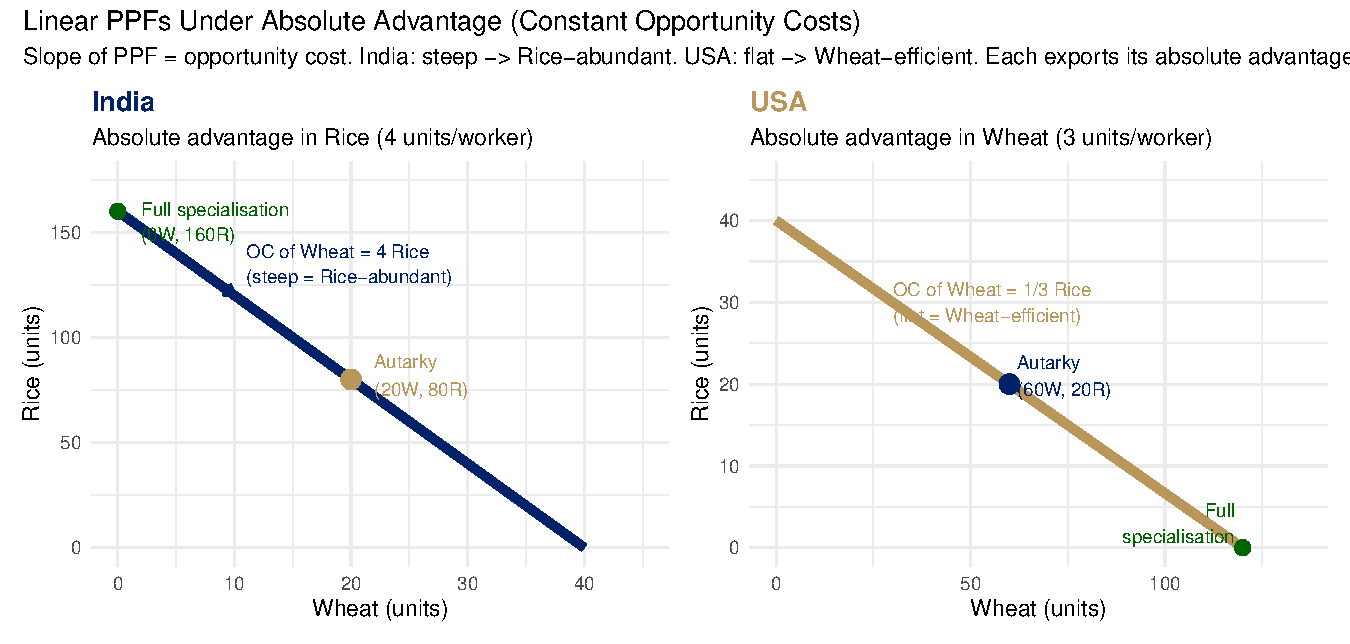
\includegraphics[keepaspectratio]{Lecture03_Theories_I_files/figure-beamer/fig-linear-ppf-1.pdf}}

}

\caption{\label{fig-linear-ppf}Linear PPFs: India and USA --- Absolute
Advantage (constant opportunity costs) Source: Author's illustration.}

\end{figure}%
\end{frame}

\begin{frame}{Gains from Trade: India and USA Under Absolute Advantage}
\phantomsection\label{gains-from-trade-india-and-usa-under-absolute-advantage}
\begin{columns}[T]
\begin{column}{0.5\linewidth}
\textbf{Without trade --- autarky (labour split 50/50)}

\begin{longtable}[]{@{}llll@{}}
\toprule\noalign{}
& India & USA & World \\
\midrule\noalign{}
\endhead
Rice (units) & 80 & 20 & \textbf{100} \\
Wheat (units) & 20 & 60 & \textbf{80} \\
\bottomrule\noalign{}
\end{longtable}

\emph{India: 20 workers × 4 = 80 Rice; 20 workers × 1 = 20 Wheat. USA:
20 × 1 = 20 Rice; 20 × 3 = 60 Wheat.}

\textbf{With trade --- full specialisation}

\begin{longtable}[]{@{}llll@{}}
\toprule\noalign{}
& India & USA & World \\
\midrule\noalign{}
\endhead
Rice (units) & \textbf{160} & 0 & \textbf{160} \\
Wheat (units) & 0 & \textbf{120} & \textbf{120} \\
\bottomrule\noalign{}
\end{longtable}

\textbf{World gains from specialisation:}

\[\Delta \text{Rice} = +60 \text{ units} \quad (+60\%)\]
\[\Delta \text{Wheat} = +40 \text{ units} \quad (+50\%)\]
\end{column}

\begin{column}{0.5\linewidth}
\textbf{Both countries can consume more after trade}

At terms of trade \textbf{2 Rice = 1 Wheat} (India exports Rice, imports
Wheat):

\begin{longtable}[]{@{}llll@{}}
\toprule\noalign{}
& Autarky & Post-trade & Gain \\
\midrule\noalign{}
\endhead
India --- Rice & 80 & 120 & \textbf{+40} \\
India --- Wheat & 20 & 20 & 0 \\
USA --- Rice & 20 & 40 & \textbf{+20} \\
USA --- Wheat & 60 & 80 & \textbf{+20} \\
\bottomrule\noalign{}
\end{longtable}

Both countries consume \textbf{outside} their individual PPFs --- trade
expands the consumption frontier beyond what each country could achieve
alone.

\textbf{Key insight:} Absolute advantage gives each nation a clear
signal about where to specialise --- the country that is objectively
more productive in a good should produce and export it.
\end{column}
\end{columns}
\end{frame}

\begin{frame}{Numerical Example: India and Bangladesh}
\phantomsection\label{numerical-example-india-and-bangladesh}
\begin{columns}[T]
\begin{column}{0.55\linewidth}
\textbf{The production possibilities}

Assume: with \textbf{1 worker-day}, each country can produce:

\begin{longtable}[]{@{}lll@{}}
\toprule\noalign{}
Country & Rice (quintals) & Jute (metres) \\
\midrule\noalign{}
\endhead
\textbf{India} & \textbf{4} & \textbf{2} \\
\textbf{Bangladesh} & \textbf{1} & \textbf{4} \\
\bottomrule\noalign{}
\end{longtable}

\textbf{Who has absolute advantage where?}

\begin{itemize}
\tightlist
\item
  \textbf{Rice:} India produces 4 Q vs Bangladesh 1 Q → {India has
  absolute advantage in rice}
\item
  \textbf{Jute:} India produces 2 M vs Bangladesh 4 M → {Bangladesh has
  absolute advantage in jute}
\end{itemize}

\textbf{Smith's recommendation:} India should export rice, Bangladesh
should export jute
\end{column}

\begin{column}{0.45\linewidth}
\textbf{Before trade (autarky)}

Assume each country has \textbf{100 worker-days} to allocate:

\begin{itemize}
\tightlist
\item
  India divides 50/50: produces 200 Q rice + 100 M jute
\item
  Bangladesh divides 50/50: produces 50 Q rice + 200 M jute
\end{itemize}

\begin{longtable}[]{@{}lll@{}}
\toprule\noalign{}
Country & Rice & Jute \\
\midrule\noalign{}
\endhead
India & 200 & 100 \\
Bangladesh & 50 & 200 \\
\textbf{World total} & \textbf{250} & \textbf{300} \\
\bottomrule\noalign{}
\end{longtable}

Now: what happens if each country \emph{fully specialises} according to
absolute advantage?
\end{column}
\end{columns}
\end{frame}

\begin{frame}{The Gains from Trade: Before and After}
\phantomsection\label{the-gains-from-trade-before-and-after}
\begin{columns}[T]
\begin{column}{0.55\linewidth}
\textbf{After full specialisation}

\begin{itemize}
\tightlist
\item
  India (100 workers all in rice): produces \textbf{400 Q rice}, 0 jute
\item
  Bangladesh (100 workers all in jute): produces 0 rice, \textbf{400 M
  jute}
\end{itemize}

\begin{longtable}[]{@{}lll@{}}
\toprule\noalign{}
Country & Rice & Jute \\
\midrule\noalign{}
\endhead
India & 400 & 0 \\
Bangladesh & 0 & 400 \\
\textbf{World total} & \textbf{400} & \textbf{400} \\
\bottomrule\noalign{}
\end{longtable}

\textbf{World production gain:}

\begin{itemize}
\tightlist
\item
  Rice: 250 → 400 (+150 Q, \textbf{+60\% increase})
\item
  Jute: 300 → 400 (+100 M, \textbf{+33\% increase})
\end{itemize}

\textbf{The world is richer} with specialisation --- this extra output
is the ``gains from trade''
\end{column}

\begin{column}{0.45\linewidth}
\textbf{Consumption after trade}

Suppose they trade at ratio \textbf{2Q rice = 2M jute} (terms of trade =
1:1):

\begin{itemize}
\tightlist
\item
  India exports 100 Q rice, imports 100 M jute
\item
  Bangladesh exports 100 M jute, imports 100 Q rice
\end{itemize}

\begin{longtable}[]{@{}lll@{}}
\toprule\noalign{}
Country & Rice (consume) & Jute (consume) \\
\midrule\noalign{}
\endhead
India & 300 & 100 \\
Bangladesh & 100 & 300 \\
\bottomrule\noalign{}
\end{longtable}

\textbf{Compare to autarky (50/50 split):}

\begin{longtable}[]{@{}lll@{}}
\toprule\noalign{}
Country & Rice gain & Jute gain \\
\midrule\noalign{}
\endhead
India & +100 (+50\%) & 0 \\
Bangladesh & +50 (+100\%) & +100 (+50\%) \\
\bottomrule\noalign{}
\end{longtable}

\textbf{Both countries consume more} of at least one good --- trade is
genuinely win-win.
\end{column}
\end{columns}
\end{frame}

\begin{frame}{India's Absolute Advantage in Agriculture}
\phantomsection\label{indias-absolute-advantage-in-agriculture}
\begin{columns}[T]
\begin{column}{0.55\linewidth}
\textbf{Where India has clear absolute advantage}

\begin{longtable}[]{@{}
  >{\raggedright\arraybackslash}p{(\linewidth - 4\tabcolsep) * \real{0.2444}}
  >{\raggedright\arraybackslash}p{(\linewidth - 4\tabcolsep) * \real{0.4222}}
  >{\raggedright\arraybackslash}p{(\linewidth - 4\tabcolsep) * \real{0.3333}}@{}}
\toprule\noalign{}
\begin{minipage}[b]{\linewidth}\raggedright
Commodity
\end{minipage} & \begin{minipage}[b]{\linewidth}\raggedright
India's global rank
\end{minipage} & \begin{minipage}[b]{\linewidth}\raggedright
Key advantage
\end{minipage} \\
\midrule\noalign{}
\endhead
Milk production & \#1 & 230M+ cattle; Operation Flood legacy \\
Pulse production & \#1 & Dryland farming expertise; diverse varieties \\
Spice production & \#1 & Tropical climate; accumulated expertise \\
Jute production & \#1 (with Bangladesh) & Ganga-Brahmaputra delta
soils \\
Rice production & \#2 (after China) & Diverse agro-climates; Green
Revolution \\
Wheat production & \#2 (after China) & Punjab-Haryana breadbasket \\
Sugarcane & \#2 (after Brazil) & Maharashtra, UP climate; Cooperative
mills \\
\bottomrule\noalign{}
\end{longtable}

\textbf{Why India has these advantages:}

\begin{itemize}
\tightlist
\item
  Diverse agro-climatic zones (12 out of 15 major global types)
\item
  Abundant agricultural labour (50\% of workforce)
\item
  Long history of cultivation → accumulated knowledge
\end{itemize}
\end{column}

\begin{column}{0.45\linewidth}
\textbf{Spices: India's oldest absolute advantage}

Spices were the original reason Europeans sought trade routes to India.
The Portuguese, Dutch, and English colonised trade routes specifically
to control the spice trade.

Today: - India produces \textasciitilde75\% of world's spices - Exports
\textasciitilde\$3.7B in spices (FY2024) - Top markets: USA, China,
Vietnam, Thailand - Key commodities: cardamom, pepper, turmeric, chilli,
cumin - 52 varieties of spices cultivated

India's spice export advantage is a textbook case of absolute advantage
based on \emph{natural resource endowments} + \emph{accumulated human
capital}.
\end{column}
\end{columns}
\end{frame}

\begin{frame}{India's Agricultural Productivity: Absolute Advantage
Indicators}
\phantomsection\label{indias-agricultural-productivity-absolute-advantage-indicators}
\begin{figure}

\centering{

\pandocbounded{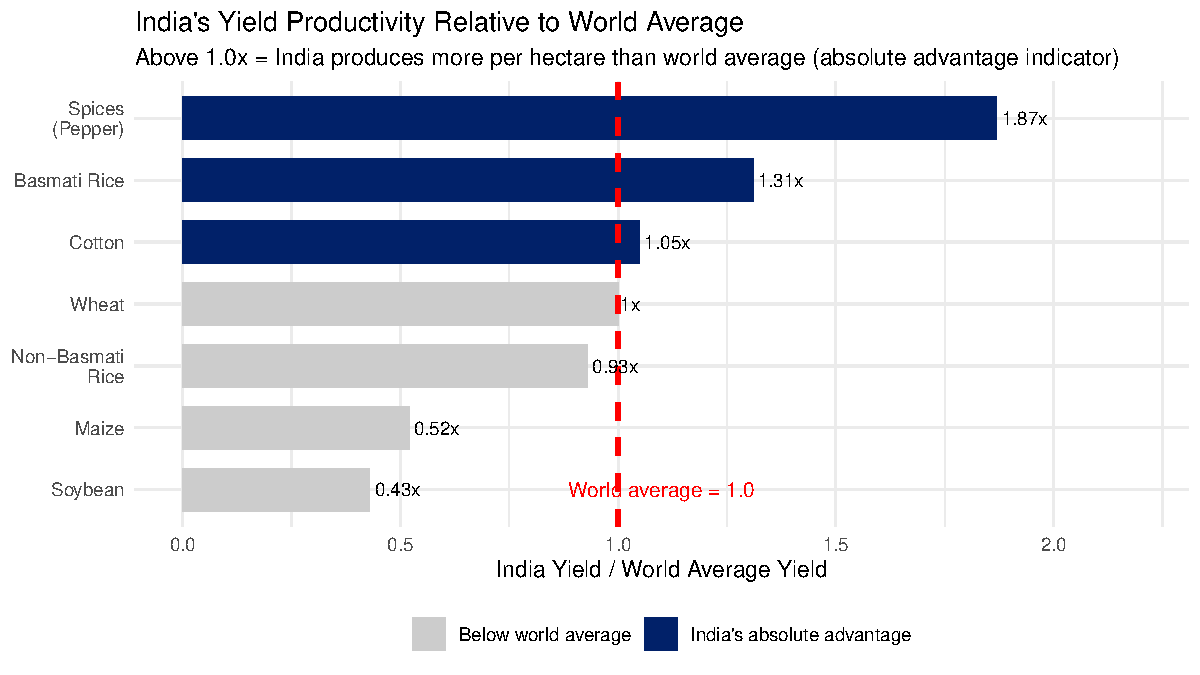
\includegraphics[keepaspectratio]{Lecture03_Theories_I_files/figure-beamer/fig-specialisation-gains-1.pdf}}

}

\caption{\label{fig-specialisation-gains}India's Yield Productivity
Relative to World Average --- Absolute Advantage Indicators Source: FAO,
FAOSTAT (2023).}

\end{figure}%

\textbf{Reading the chart:} Spices (Pepper) at 1.87x and Basmati Rice at
1.31x show the strongest absolute advantage --- India produces far more
per hectare than the world average. Maize (0.52x) and Soybean (0.43x)
show India well below world average --- not where export effort should
be directed. Cotton (1.05x) and Non-Basmati Rice (0.93x) are near parity
--- other factors (price, quality, logistics) determine trade patterns.
\end{frame}

\begin{frame}{Limitations of Absolute Advantage Theory}
\phantomsection\label{limitations-of-absolute-advantage-theory}
\begin{columns}[T]
\begin{column}{0.5\linewidth}
\textbf{Theoretical limitations}

\begin{enumerate}
\tightlist
\item
  \textbf{Ignores the case where one country is better at everything}
  --- If India has absolute advantage in \emph{both} rice and jute,
  Smith's theory says Bangladesh should not trade → clearly wrong
\item
  \textbf{Labour-only model} --- Ignores capital, land, technology;
  these matter enormously in agriculture
\item
  \textbf{Constant returns to scale} --- Real agriculture has
  diminishing returns (limited fertile land); opportunity costs
  \emph{increase} as production expands
\item
  \textbf{Full employment assumption} --- In reality, India has seasonal
  unemployment; trade may employ idle labour rather than divert it
\end{enumerate}
\end{column}

\begin{column}{0.5\linewidth}
\textbf{Practical limitations}

\begin{enumerate}
\setcounter{enumi}{4}
\tightlist
\item
  \textbf{Transport costs are ignored} --- A commodity with a slight
  absolute advantage may not be worth trading if freight cost is high
  (bulk grains)
\item
  \textbf{No room for trade policy} --- The model says free trade is
  always optimal; ignores infant industry, food security, strategic
  goods arguments
\item
  \textbf{No product quality differences} --- India exports basmati rice
  (premium quality) and non-basmati (commodity); absolute advantage
  theory treats all rice as identical
\item
  \textbf{Static model} --- Absolute advantage can change over time
  (South Korea had no absolute advantage in electronics in 1960; now it
  does)
\end{enumerate}
\end{column}
\end{columns}
\end{frame}

\begin{frame}{The Problem with Absolute Advantage}
\phantomsection\label{the-problem-with-absolute-advantage}
\begin{columns}[T]
\begin{column}{0.6\linewidth}
\textbf{The critical case: What if one country is better at everything?}

Suppose USA vs India:

\begin{longtable}[]{@{}lll@{}}
\toprule\noalign{}
Country & Wheat (tonnes/worker) & Software (units/worker) \\
\midrule\noalign{}
\endhead
\textbf{USA} & \textbf{4} & \textbf{8} \\
\textbf{India} & \textbf{2} & \textbf{2} \\
\bottomrule\noalign{}
\end{longtable}

USA has absolute advantage in \textbf{both} wheat and software.

\textbf{Smith's theory predicts:} No basis for trade --- India has no
absolute advantage in anything.

\textbf{But we \emph{know} India and USA trade extensively!}

\begin{itemize}
\tightlist
\item
  India exports software services to USA (\$80--100B/year)
\item
  India exports agricultural products to USA
\end{itemize}

\textbf{Smith's theory cannot explain this. Something deeper is at
work.}
\end{column}

\begin{column}{0.4\linewidth}
\textbf{What Smith missed}

The key is not absolute productivity but \textbf{relative} (or
comparative) productivity.

Even though USA is better at \emph{both} goods, the \emph{degree} of
advantage differs:

\begin{itemize}
\tightlist
\item
  USA is 2× better at wheat (4 vs 2)
\item
  USA is \textbf{4× better} at software (8 vs 2)
\end{itemize}

USA has a \emph{stronger} advantage in software → USA should specialise
in software

India has a \emph{lesser} disadvantage in wheat → India should
specialise in wheat

This is \textbf{comparative advantage} --- David Ricardo's great
insight.

We will prove this formally in \textbf{Lecture 4} --- but the intuition
is: even the worst player on a sports team should play the position
they're \emph{least bad} at.
\end{column}
\end{columns}
\end{frame}

\begin{frame}{Smith vs Mercantilism: A Summary Comparison}
\phantomsection\label{smith-vs-mercantilism-a-summary-comparison}
\begin{longtable}[]{@{}
  >{\raggedright\arraybackslash}p{(\linewidth - 4\tabcolsep) * \real{0.1964}}
  >{\raggedright\arraybackslash}p{(\linewidth - 4\tabcolsep) * \real{0.2321}}
  >{\raggedright\arraybackslash}p{(\linewidth - 4\tabcolsep) * \real{0.5714}}@{}}
\toprule\noalign{}
\begin{minipage}[b]{\linewidth}\raggedright
Dimension
\end{minipage} & \begin{minipage}[b]{\linewidth}\raggedright
Mercantilism
\end{minipage} & \begin{minipage}[b]{\linewidth}\raggedright
Adam Smith (Absolute Advantage)
\end{minipage} \\
\midrule\noalign{}
\endhead
\textbf{Source of national wealth} & Stock of gold and silver &
Productive capacity; goods and services \\
\textbf{Nature of trade} & Zero-sum (one country's gain = another's
loss) & Win-win (both countries gain from specialisation) \\
\textbf{Objective of trade policy} & Maximise exports; minimise imports
& Maximise specialisation; allow free exchange \\
\textbf{Role of government} & Active: subsidise exports, restrict
imports, grant monopolies & Minimal: allow markets to direct
specialisation \\
\textbf{Imports: good or bad?} & Bad --- gold flows out & Good ---
access to cheaper goods; frees resources for comparative advantage
sectors \\
\textbf{Trade balance} & Surplus is the goal & Irrelevant; what matters
is consumption possibilities \\
\textbf{Colonies} & Essential --- raw material source + captive market &
Unnecessary and harmful to the coloniser too (waste of resources) \\
\textbf{Legacy} & Colonial trade systems; modern currency wars &
Foundation of free trade economics; WTO ideology \\
\bottomrule\noalign{}
\end{longtable}
\end{frame}

\section{Part IV: India Policy
Applications}\label{part-iv-india-policy-applications}

\begin{frame}{India Policy Application: Mercantilism vs Smith in Real
Decisions}
\phantomsection\label{india-policy-application-mercantilism-vs-smith-in-real-decisions}
\begin{columns}[T]
\begin{column}{0.55\linewidth}
\textbf{The rice export ban (2023): a case study}

\emph{The mercantilist argument for the ban:} - Domestic rice prices
rising → risk food inflation rising → protect domestic consumers - Keep
rice in India → ensure food security → classic mercantilist hoarding of
``strategic resources''

\emph{The Smithian argument against the ban:} - India has absolute (and
comparative) advantage in rice → should be \emph{exporting}, not
restricting - Ban reduces income of 30 million paddy farmers - Ban
damages long-term export relationships with Bangladesh, Africa - Ban
causes global price spike → India blamed for food security crisis in
import-dependent countries

\textbf{Who won?} The ban was implemented in August 2023 ---
mercantilist/food security logic prevailed over free trade logic.
\end{column}

\begin{column}{0.45\linewidth}
\textbf{The deeper tension}

India's trade policy in agriculture oscillates between two poles:

\textbf{Export restrictionism} (mercantilist): Rice ban, wheat ban,
sugar export quotas, onion export bans

\textbf{Export promotion} (Smithian): FTP 2023--28, APEDA support,
RoDTEP, agri-export zones

Both impulses co-exist because the political economy is complex:
consumers want cheap food; farmers want high prices; the government
wants foreign exchange; WTO wants compliance.

There is no simple answer --- which is why studying trade theory is so
important.
\end{column}
\end{columns}
\end{frame}

\begin{frame}{The Case of Indian Spices: Absolute Advantage in Action}
\phantomsection\label{the-case-of-indian-spices-absolute-advantage-in-action}
\begin{columns}[T]
\begin{column}{0.6\linewidth}
\textbf{India's dominance in global spice markets}

\begin{itemize}
\tightlist
\item
  \textbf{Production:} India produces 75\% of world's spices by volume;
  50\%+ by value
\item
  \textbf{Export performance (FY2024):} \$3.7 billion; 14\% growth over
  FY2023
\item
  \textbf{Volume:} \textasciitilde2.1 million tonnes exported
\end{itemize}

\textbf{Top commodities and destinations}

\begin{longtable}[]{@{}lll@{}}
\toprule\noalign{}
Spice & Export value & Top markets \\
\midrule\noalign{}
\endhead
Chilli & \$982M & USA, Vietnam, Sri Lanka \\
Cumin & \$700M & USA, Bangladesh, China \\
Cardamom & \$350M & Saudi Arabia, UAE \\
Turmeric & \$300M & Bangladesh, USA \\
Pepper & \$190M & USA, Vietnam \\
\bottomrule\noalign{}
\end{longtable}

\textbf{Source of absolute advantage:} Specific agro-climatic conditions
(Kerala for pepper/cardamom, AP/Rajasthan for chilli/cumin, Tamil Nadu
for turmeric) that cannot be replicated at comparable cost elsewhere
\end{column}

\begin{column}{0.4\linewidth}
\textbf{The spice trade: history and economics}

Ancient trade routes from India → Arabian Peninsula → Mediterranean
existed for 3,000+ years. Roman records mention importing pepper from
India at high prices.

The search for direct sea routes to India's spice markets was the
primary driver of the ``Age of Exploration'' --- Columbus was looking
for a route to India's spices when he accidentally reached the Americas.

Today, India's spice exports are still driven by the same absolute
advantage: climate, soils, and accumulated expertise that competitors
cannot easily replicate.
\end{column}
\end{columns}
\end{frame}

\begin{frame}{Summary: Mercantilism and Absolute Advantage}
\phantomsection\label{summary-mercantilism-and-absolute-advantage}
\textbf{Key points from Lecture 3}

\textbf{Mercantilism (1500--1750):} - Wealth = gold; goal = trade
surplus; trade is zero-sum - Led to colonial exploitation, including
India's ``drain of wealth'' - Critiqued by Hume (price-specie-flow) and
Smith (wealth is production, not gold) - Modern echoes: export bans,
currency manipulation, FTP export targets

\textbf{Absolute Advantage (Adam Smith, 1776):} - Each country should
specialise in what it produces most efficiently - Trade is win-win ---
world production rises with specialisation - India and Bangladesh
example: rice vs jute, both gain from specialisation - India's
agricultural absolute advantages: rice, spices, pulses, milk --- rooted
in climate, labour, and accumulated knowledge

\textbf{The fatal limitation:} What if one country is better at
\emph{everything}? Smith cannot explain trade between USA and India.
This is the gap Ricardo fills with \textbf{comparative advantage}.
\end{frame}

\begin{frame}{Key Takeaways: Lecture 3}
\phantomsection\label{key-takeaways-lecture-3}
\textbf{What we covered today}

\begin{itemize}
\tightlist
\item
  \textbf{Mercantilism:} Trade as power accumulation; maximise surplus;
  zero-sum worldview → systematically flawed, but echoes persist in
  modern policy
\item
  \textbf{Colonial trade in India:} British mercantilism extracted
  surplus, destroyed Indian textile industry, contributed to Indian
  poverty → ``drain of wealth'' (Naoroji)
\item
  \textbf{Hume and Smith's critiques:} Trade surpluses are
  self-correcting (price-specie-flow); real wealth is productive
  capacity, not gold
\item
  \textbf{Absolute advantage:} Specialise in what you produce with
  highest \emph{absolute} efficiency; trade is win-win → both India and
  Bangladesh can gain from specialisation in rice and jute
\item
  \textbf{India's absolute advantages:} Rice, spices, pulses, milk, jute
  --- rooted in agro-climatic endowments and accumulated human capital
\item
  \textbf{Fundamental limitation:} Absolute advantage cannot explain
  trade when one country is more efficient in \emph{everything} → sets
  up Ricardo's comparative advantage
\end{itemize}
\end{frame}

\begin{frame}{Next Lecture: Lecture 4}
\phantomsection\label{next-lecture-lecture-4}
\begin{columns}[T]
\begin{column}{0.6\linewidth}
\textbf{Theories of International Trade II --- Comparative Advantage}
\emph{(May 19, 2026)}

We will cover:

\begin{itemize}
\tightlist
\item
  \textbf{David Ricardo (1817):} The most profound insight in economics
  --- comparative advantage
\item
  \textbf{The opportunity cost logic:} Why the \emph{relative} cost, not
  absolute cost, determines trade patterns
\item
  \textbf{Formal model:} Two countries, two goods, with full numerical
  derivation
\item
  \textbf{India vs USA example:} Why India exports software services
  despite USA being more productive in absolute terms
\item
  \textbf{Production Possibility Frontier (PPF):} Formal diagrammatic
  treatment
\item
  \textbf{The gains from trade:} Measured precisely with PPF and
  consumption possibilities
\item
  \textbf{Empirical evidence:} Does the Ricardian model predict actual
  trade patterns?
\end{itemize}
\end{column}

\begin{column}{0.4\linewidth}
\textbf{Suggested reading}

\begin{itemize}
\tightlist
\item
  Krugman, Obstfeld \& Melitz, \emph{International Economics}, Ch. 3
\item
  Ricardo, D. (1817). \emph{Principles of Political Economy and
  Taxation}, Ch. 7 (excerpt)
\item
  Goldin, I. and Reinert, K. (2012). \emph{Globalization for
  Development}, Ch. 2
\end{itemize}

\textbf{Key question to prepare:}

If India is only half as productive as the USA in \emph{all}
agricultural commodities, should India and USA trade at all? If yes,
\emph{what} should each produce?
\end{column}
\end{columns}
\end{frame}

\section{Appendix}\label{appendix}

\begin{frame}{Additional Resources}
\phantomsection\label{additional-resources}
\begin{columns}[T]
\begin{column}{0.5\linewidth}
\textbf{Further Reading}

\begin{itemize}
\tightlist
\item
  \emph{International Economics} --- Salvatore (Ch. 2-3)
\item
  \emph{International Economics} --- Appleyard \& Field (Ch. 2-3)
\item
  RBI/DGCI\&S/APEDA databases for latest data
\end{itemize}
\end{column}

\begin{column}{0.5\linewidth}
\textbf{Key Data Sources}

\begin{itemize}
\tightlist
\item
  DGCI\&S: India's merchandise trade
\item
  RBI: Balance of payments data\\
\item
  APEDA: Agricultural export statistics
\item
  WTO: Tariff and trade databases
\end{itemize}
\end{column}
\end{columns}
\end{frame}




\end{document}
